\begin{figure}[H]
    \centering
        \centering
        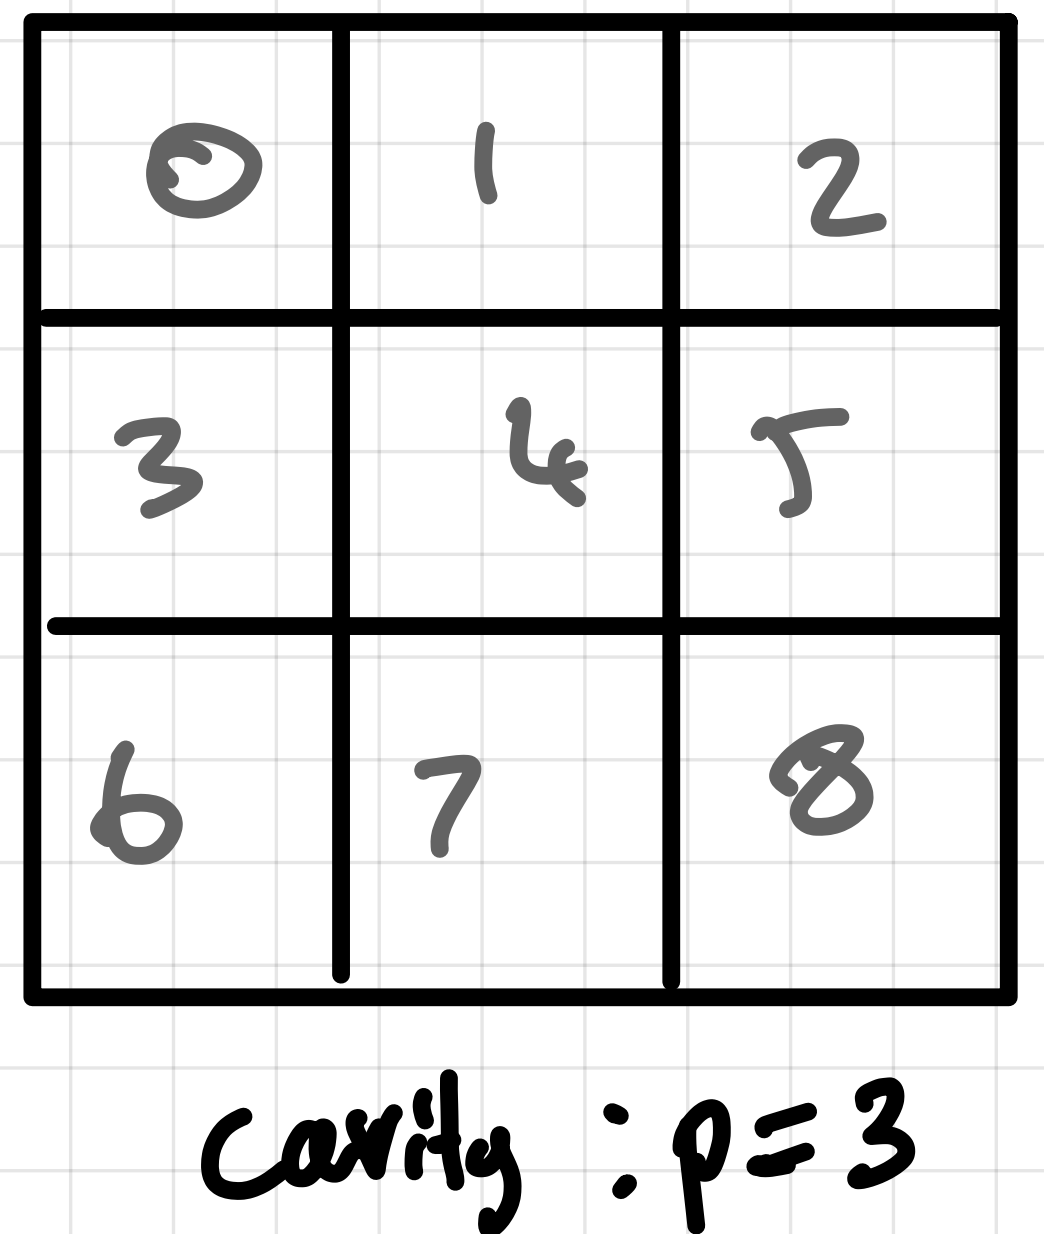
\includegraphics[width=0.45\linewidth]{Images/VirtualTopology.png}
        \caption{Virtual topology of MPI ranks}
        \label{fig:VirtualTopology}

\end{figure}



\begin{figure}[H]
    \centering
    \rotatebox{270}{%
        \begin{minipage}{\textheight}
            \vspace{1cm}
            \verbatiminput{../report/Data/timings.txt}
            \vspace*{2cm}
            \caption{``timings.txt'' to show sample data for scaling plot}
            \label{fig:timings} % Place the \label command after \caption
        \end{minipage}%
    }
\end{figure}

\begin{figure}[H]
    \centering
        \centering
        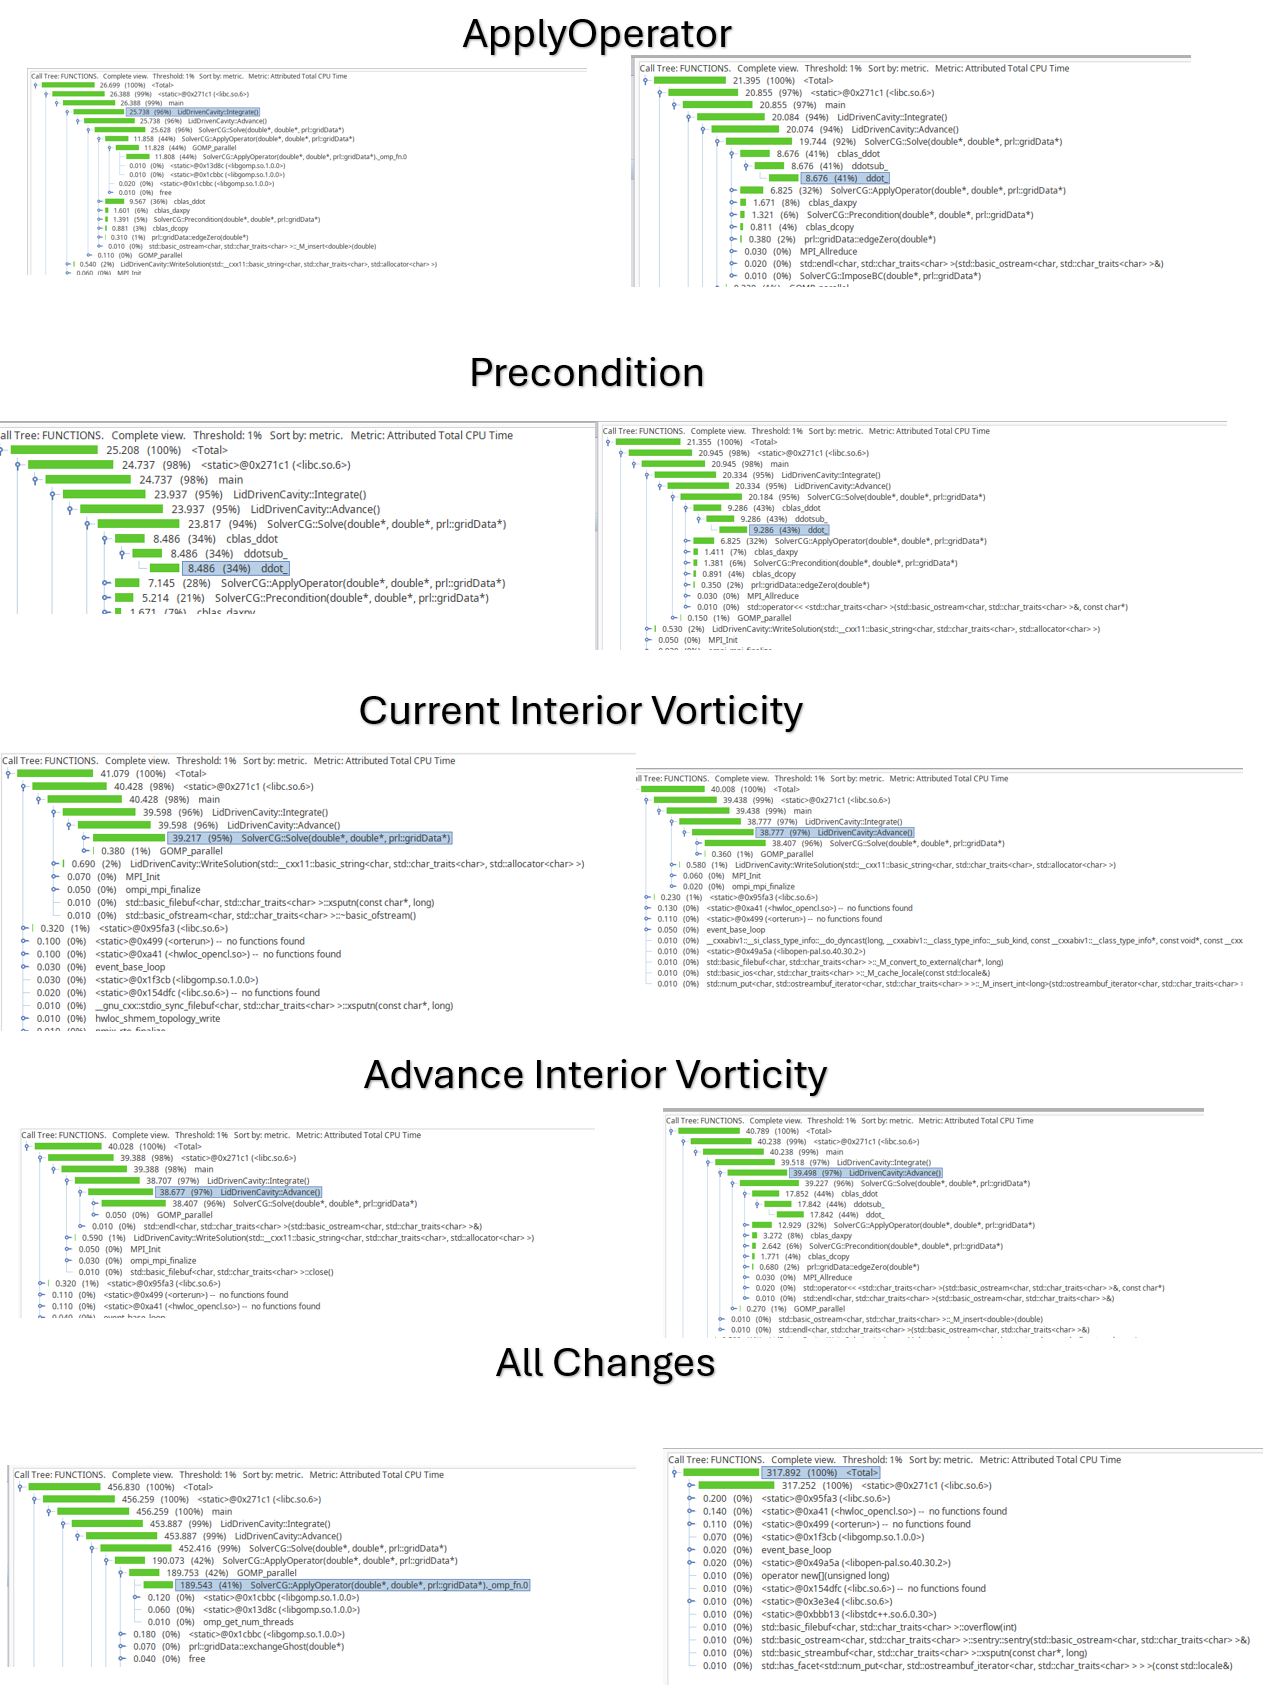
\includegraphics[width=\linewidth]{Images/optim.png}
        \caption{Call trees showing inclusive times for profiling}
        \label{fig:optim}

\end{figure}


\begin{figure}[H]
    \centering
    \begin{subfigure}[b]{0.45\textwidth}
        \centering
        \includegraphics[width=\textwidth]{Images/\largedomain___MPIVINIT.png}
        \caption{Initialise}
        \label{fig:large:MPIVINIT}
    \end{subfigure}
    \hfill
    \begin{subfigure}[b]{0.45\textwidth}
        \centering
        \includegraphics[width=\textwidth]{Images/\largedomain___MPIVIC.png}
        \caption{Write Initial Conditions}
        \label{fig:large:MPIVIC}
    \end{subfigure}
    \\
    \begin{subfigure}[b]{0.45\textwidth}
        \centering
        \includegraphics[width=\textwidth]{Images/\largedomain___MPIVSOLVE.png}
        \caption{Solve}
        \label{fig:large:MPIVSOLVE}
    \end{subfigure}
    \hfill
    \begin{subfigure}[b]{0.45\textwidth}
        \centering
        \includegraphics[width=\textwidth]{Images/\largedomain___MPIVFINAL.png}
        \caption{Write Final Conditions}
        \label{fig:large:MPIVFINAL}
    \end{subfigure}
    \caption{Plots showing effect of MPI parallelisation on various functions for the ``Large'' settings}
    \label{fig:large:MPI}
\end{figure}

\begin{figure}[H]
    \centering
    \begin{subfigure}[b]{0.45\textwidth}
        \centering
        \includegraphics[width=\textwidth]{Images/\largedomain___OMPVINIT.png}
        \caption{Initialise}
        \label{fig:large:OMPVINIT}
    \end{subfigure}
    \hfill
    \begin{subfigure}[b]{0.45\textwidth}
        \centering
        \includegraphics[width=\textwidth]{Images/\largedomain___OMPVIC.png}
        \caption{Write Initial Conditions}
        \label{fig:large:OMPVIC}
    \end{subfigure}
    \\
    \begin{subfigure}[b]{0.45\textwidth}
        \centering
        \includegraphics[width=\textwidth]{Images/\largedomain___OMPVSOLVE.png}
        \caption{Solve}
        \label{fig:large:OMPVSOLVE}
    \end{subfigure}
    \hfill
    \begin{subfigure}[b]{0.45\textwidth}
        \centering
        \includegraphics[width=\textwidth]{Images/\largedomain___OMPVFINAL.png}
        \caption{Write Final Conditions}
        \label{fig:large:OMPVFINAL}
    \end{subfigure}
    \caption{Plots showing effect of Open MP parallelisation on various functions for the ``Large'' settings}
    \label{fig:large:OMP}
\end{figure}

\begin{figure}[H]
    \centering
    \begin{subfigure}[b]{0.45\textwidth}
        \centering
        \includegraphics[width=\textwidth]{Images/\smalldomain___MPIVINIT.png}
        \caption{Initialise}
        \label{fig:small:MPIVINIT}
    \end{subfigure}
    \hfill
    \begin{subfigure}[b]{0.45\textwidth}
        \centering
        \includegraphics[width=\textwidth]{Images/\smalldomain___MPIVIC.png}
        \caption{Write Initial Conditions}
        \label{fig:small:MPIVIC}
    \end{subfigure}
    \\
    \begin{subfigure}[b]{0.45\textwidth}
        \centering
        \includegraphics[width=\textwidth]{Images/\smalldomain___MPIVSOLVE.png}
        \caption{Solve}
        \label{fig:small:MPIVSOLVE}
    \end{subfigure}
    \hfill
    \begin{subfigure}[b]{0.45\textwidth}
        \centering
        \includegraphics[width=\textwidth]{Images/\smalldomain___MPIVFINAL.png}
        \caption{Write Final Conditions}
        \label{fig:small:MPIVFINAL}
    \end{subfigure}
    \caption{Plots showing effect of MPI parallelisation on various functions for the ``Small'' settings}
    \label{fig:small:MPI}
\end{figure}

\begin{figure}[H]
    \centering
    \begin{subfigure}[b]{0.45\textwidth}
        \centering
        \includegraphics[width=\textwidth]{Images/\smalldomain___OMPVINIT.png}
        \caption{Initialise}
        \label{fig:small:OMPVINIT}
    \end{subfigure}
    \hfill
    \begin{subfigure}[b]{0.45\textwidth}
        \centering
        \includegraphics[width=\textwidth]{Images/\smalldomain___OMPVIC.png}
        \caption{Write Initial Conditions}
        \label{fig:small:OMPVIC}
    \end{subfigure}
    \\
    \begin{subfigure}[b]{0.45\textwidth}
        \centering
        \includegraphics[width=\textwidth]{Images/\smalldomain___OMPVSOLVE.png}
        \caption{Solve}
        \label{fig:small:OMPVSOLVE}
    \end{subfigure}
    \hfill
    \begin{subfigure}[b]{0.45\textwidth}
        \centering
        \includegraphics[width=\textwidth]{Images/\smalldomain___OMPVFINAL.png}
        \caption{Write Final Conditions}
        \label{fig:small:OMPVFINAL}
    \end{subfigure}
    \caption{Plots showing effect of Open MP parallelisation on various functions for the ``Small'' settings}
    \label{fig:small:OMP}
\end{figure}